%%%%%%%%%%%%%%%%%%%%%%%%%%%%%%%%%%%%%%%%%
% Masters/Doctoral Thesis
% LaTeX Template
% Version 2.5 (27/8/17)
%
% This template was downloaded from:
% http://www.LaTeXTemplates.com
%
% Version 2.x major modifications by:
% Vel (vel@latextemplates.com)
%
% This template is based on a template by:
% Steve Gunn (http://users.ecs.soton.ac.uk/srg/softwaretools/document/templates/)
% Sunil Patel (http://www.sunilpatel.co.uk/thesis-template/)
%
% Template license:
% CC BY-NC-SA 3.0 (http://creativecommons.org/licenses/by-nc-sa/3.0/)
%
%%%%%%%%%%%%%%%%%%%%%%%%%%%%%%%%%%%%%%%%%

%----------------------------------------------------------------------------------------
%	PACKAGES AND OTHER DOCUMENT CONFIGURATIONS
%----------------------------------------------------------------------------------------

\documentclass[
11pt, % The default document font size, options: 10pt, 11pt, 12pt
%oneside, % Two side (alternating margins) for binding by default, uncomment to switch to one side
english, % ngerman for German
singlespacing, % Single line spacing, alternatives: onehalfspacing or doublespacing
%draft, % Uncomment to enable draft mode (no pictures, no links, overfull hboxes indicated)
%nolistspacing, % If the document is onehalfspacing or doublespacing, uncomment this to set spacing in lists to single
%liststotoc, % Uncomment to add the list of figures/tables/etc to the table of contents
%toctotoc, % Uncomment to add the main table of contents to the table of contents
%parskip, % Uncomment to add space between paragraphs
%nohyperref, % Uncomment to not load the hyperref package
headsepline, % Uncomment to get a line under the header
%chapterinoneline, % Uncomment to place the chapter title next to the number on one line
%consistentlayout, % Uncomment to change the layout of the declaration, abstract and acknowledgements pages to match the default layout,
]{article} % The class file specifying the document structure

\usepackage[utf8]{inputenc} % Required for inputting international characters
\usepackage[T1]{fontenc} % Output font encoding for international characters
\usepackage{textcomp}

\usepackage{mathpazo} % Use the Palatino font by default

\usepackage[%
    backend=biber,style=authoryear-icomp,sorting=nyt,maxbibnames=100,%
    bibencoding=utf8,natbib,uniquelist=false,uniquename=false,maxcitenames=2,ibidtracker=false]{biblatex} % Use the bibtex backend with the authoryear citation style (which resembles APA)

\addbibresource{mybib.bib} % The filename of the bibliography
\addbibresource{psy-view.bib} % The filename of the bibliography

\usepackage[autostyle=true]{csquotes} % Required to generate language-dependent quotes in the bibliography
\usepackage{geometry}
\usepackage{xcolor} % Required for specifying custom colours

%----------------------------------------------------------------------------------------
%	MARGIN SETTINGS
%----------------------------------------------------------------------------------------

\geometry{
	paper=a4paper, % Change to letterpaper for US letter
	inner=1.5cm, % Inner margin
	outer=1.8cm, % Outer margin
	bindingoffset=.5cm, % Binding offset
	top=1.5cm, % Top margin
	bottom=1.5cm, % Bottom margin
	marginparwidth=2.5cm,
	%showframe, % Uncomment to show how the type block is set on the page
}

\colorlet{mdtRed}{red!50!black}

%----------------------------------------------------------------------------------------
%	THESIS INFORMATION
%----------------------------------------------------------------------------------------

\title{Psyplot - Sustainable coding within a flexible framework} % Your thesis title, this is used in the title and abstract, print it elsewhere with \ttitle examiner's name, this is not currently used anywhere in the template, print it elsewhere with \examname
\author{Philipp S. \textsc{Sommer}} % Your name, this is used in the title page and abstract, print it elsewhere with \authorname


\AtBeginDocument{
\hypersetup{pdftitle=Psyplot - Sustainable coding within a flexible framework} % Set the PDF's title to your title
\hypersetup{pdfauthor=Philipp S. Sommer} % Set the PDF's author to your name
\hypersetup{pdfkeywords=Climate Science} % Set the PDF's keywords to your keywords
\hypersetup{pdfpagemode={UseOutlines},
pdfpagelabels,pagebackref,plainpages=false,
bookmarksopen=true,
bookmarksopenlevel=0,
hypertexnames=false,
colorlinks=true,% Set to false to disable coloring links
citecolor=magenta,% The color of citations
linkcolor=mdtRed,% The color of references to document elements (sections, figures, etc)
urlcolor=mdtRed,% The color of hyperlinks (URLs)
pdfstartview={FitV},
unicode,
breaklinks=true,
}
}

%----------------------------------------------------------------------------------------
%	CUSTOM LATEX PACKAGES
%----------------------------------------------------------------------------------------
\usepackage{tikz}
\usepackage{appendix}
\usepackage{amsmath}
\usepackage{algorithmic}
\usepackage{algorithm}
\usepackage{hyperref}
\usepackage{fancyvrb}
\usepackage[acronym,toc,nomain,savenumberlist]{glossaries}
\usepackage[colorinlistoftodos,textsize=tiny,disable]{todonotes}
\usepackage{titlesec, titletoc}  % necessary for putting bars and labels under the part in toc
\usepackage{multirow}
\usepackage{longtable}
\usepackage{afterpage}
\usepackage{pdfpages}
\usepackage{booktabs}
\usepackage{wrapfig}

\setcounter{biburllcpenalty}{7000}
\setcounter{biburlucpenalty}{8000}

\input{pygments-header.tex}

%----------------------------------------------------------------------------------------
%	CUSTOM LATEX COMMANDS
%----------------------------------------------------------------------------------------

\newcommand\Chapter[3][false]{
	\ifthenelse{\equal{#1}{false}} {%
		\chapter[#2: {\itshape#3}]{#2\\[2ex]\Large\itshape#3}
	}{%
		\chapter[#1]{#2\\[2ex]\Large\itshape#3}
	}
}
\newcommand\tophline{\hline\noalign{\vspace{1mm}}}
\newcommand\middlehline{\noalign{\vspace{1mm}}\hline\noalign{\vspace{1mm}}}
\newcommand\bottomhline{\noalign{\vspace{1mm}}\hline}
\newcommand\hhline{\noalign{\vspace{1mm}}\hline\noalign{\vspace{1mm}}}
\DeclareRobustCommand*\unit[1]%
{\ensuremath{%
		{\thinmuskip3mu\relax
			\def\mu{\text{\textmu}}\def~{\,}%
			\ifx\f@series\testbx\mathbf{#1}\else\mathrm{#1}\fi}}}

\newcounter{addrefcounter}

\newcommand{\addref}[1][]{\stepcounter{addrefcounter}\todo[color=red!40]{\theaddrefcounter: Add reference. #1}}
\newcommand{\rewrite}[1]{\todo[color=green!40, size=\normalsize, inline]{#1}}

\newcommand{\bibforkey}[1]{%
	\defbibcheck{key#1}{
		\iffieldequalstr{entrykey}{#1}
		{}
		{\skipentry}}%
	\printbibliography[heading=none,check=key#1]%
}

% put bars and labels under the part in toc
\titlelabel{\thetitle\quad}

\titlecontents{part}%
[0pt]{\bfseries\large\protect\addvspace{4ex}}
{}{\partname~}
{\hfill\contentspage}%
[\addvspace{0.3ex}\titlerule\addvspace{1.5ex}]%

\makeatletter
\def\convertto#1#2{\strip@pt\dimexpr #2*65536/\number\dimexpr 1#1}
\makeatother

%----------------------------------------------------------------------------------------
%	ABBREVIATIONS
%----------------------------------------------------------------------------------------

\makenoidxglossaries

\newacronym{esm}{ESM}{Earth System Model}
\newacronym{gcm}{GCM}{General Circulation Model}
\newacronym{nao}{NAO}{North Atlantic Oscillation}
\newacronym{pmip}{PMIP}{Paleoclimate Modelling Intercomparison Project}
\newacronym{cmip}{CMIP}{Coupled Model Intercomparison Project}
\newacronym{ipcc}{IPCC}{Intergovernmental Panel on Climate Change}
\newacronym{epd}{EPD}{European Pollen Database}
\newacronym{napd}{NAPD}{North American Pollen Database}
\newacronym{empd}{EMPD}{Eurasian Modern Pollen Database}
\newacronym{noaa}{NOAA}{National Oceanic and Atmospheric Administration}
\newacronym{ncdc}{NCDC}{National Climatic Data Center}
\newacronym{mpi-esm}{MPI-ESM-LR}{Max-Planck-Insitute Earth System Model at low resolution}
\newacronym{htm}{HTM}{Holocene Thermal Maximum}
\newacronym{lig}{LIG}{Last Interglacial}
\newacronym{lgm}{LGM}{Last Glacial Maximum}
\newacronym{cdo}{CDO}{Climate Data Operator}
\newacronym{nco}{NCO}{netCDF Operator}
\newacronym{foss}{FOSS}{Free and Open-Source Software}
\newacronym{ci}{CI}{Continuous Integration}
\newacronym{api}{API}{Application programming interface}
\newacronym{gui}{GUI}{graphical user interface}
\newacronym[longplural={Earth System Models of Intermediate Complexity}]{emic}{EMIC}{Earth System Model of Intermediate Complexity}
\newacronym{jja}{JJA}{summer (June, July and August)}
\newacronym{djf}{DJF}{winter (December, January and February)}
\newacronym{mat}{MAT}{modern analogue technique}
\newacronym{gam}{GAM}{Generalized Additive Model}
\newacronym{mcmc}{MCMC}{Markov chain Monte Carlo}
\newacronym{lapd}{LAPD}{Latin American Pollen Database}
\newacronym{apd}{APD}{African Pollen Database}

\includeonly{Chapters/psyplot-submission}

\begin{document}

%\frontmatter % Use roman page numbering style (i, ii, iii, iv...) for the pre-content pages

\pagestyle{plain} % Default to the plain heading style until the thesis style is called for the body content

%----------------------------------------------------------------------------------------
%	TITLE PAGE
%----------------------------------------------------------------------------------------

%\cleardoublepage
%\addcontentsline{toc}{chapter}{Imprimatur}
%\includepdf{imprimatur.pdf}
%
%\cleardoublepage

%----------------------------------------------------------------------------------------
%	LIST OF CONTENTS/FIGURES/TABLES PAGES
%----------------------------------------------------------------------------------------

%\tableofcontents % Prints the main table of contents

%----------------------------------------------------------------------------------------
%	THESIS CONTENT - CHAPTERS
%----------------------------------------------------------------------------------------

%\mainmatter % Begin numeric (1,2,3...) page numbering

% Include the chapters of the thesis as separate files from the Chapters folder
% Uncomment the lines as you write the chapters
\maketitle

\begin{refsection}

%----------------------------------------------------------------------------------------
%	SECTION 1
%----------------------------------------------------------------------------------------

\section{Introduction}  \label{sec:psyplot-review}

A fundamental challenge for scientific code is the reproducibility. Being untrained programmers, scientists usually do not follow a systematic framework. The generated scripts usually need to be adapted every time a new project starts. This makes the analysis difficult to share with other researchers and the general public. The open-source psyplot software wants to generalize this data processing and visualization steps by providing a framework that is highly flexible, interoperates with standard computational data processing tools and enables flexible visualizations and adaptations. The software aims to motivate researchers to split their analysis into so-called “formatoptions”, that act as little units within a configurable data analysis pipeline (a so-called “plotter”). These formatoptions can then easily be used in a convenient high-level python API and a graphical user interface. A templating formalism for plugins further facilitates the distribution of the methodology as python packages.

The framework is written in the programming language Python \citep{PerezGrangerHunter2011} and the current functionalities build upon the visualization package \textit{matplotlib} \citep{Hunter2007} and the N-dimensional array processing package \textit{xarray} \citep{HoyerHamman2017}, that closely interoperate with the numeric packages numpy and scipy \citep{JonesOliphantPetersonEtAl2001, Oliphant2006} and the parallel computing library dask \citep{DDT2016}. Due to the flexibility of Python, it can be used from the command-line, a \gls{gui} (section \ref{sec:psyplot-gui}) or jupyter notebooks\footnote{\url{https://jupyter.org/}} \citep{KluyverRaganKelleyPerezEtAl2016}.

Our plugin-based and modular approach encourages scientists to develop more sustainable research software and to makes it available to other scientists.

The remaining part of this document provides an overview of the framework with its data model, plugins and the \gls{gui}. More information about usage, implementation examples and adaptations of the framework\footnote{\url{https://psyplot.github.io/examples/general/example_extending_psyplot.html}} can be found in the online documentation at \url{https://psyplot.github.io}.

\section*{Side note}

psyplot has been developed as a side project within the PhD-Thesis \cite{Sommer2020e} at the University of Lausanne, Switzerland. Most of the text in this document has been extracted from this chapter. psyplot is now further maintained and developed by Philipp S. Sommer at the Helmholtz-Zentrum Hereon.

\section{The psyplot framework}  \label{sec:psyplot-framework}

The psyplot framework consists of three parts: The core structure that is built upon \textit{xarray} and provides the general infrastructure (section \ref{sec:psyplot-core}), the plugins that use the plotting functionalities of \textit{matplotlib} (section \ref{sec:psyplot-plugins}), and the \gls{gui} (section \ref{sec:psyplot-gui}).


\subsection{Psyplot core structure}  \label{sec:psyplot-core}

The core structure of psyplot consists of five base classes that interact with each other, the visualization objects \textit{Plotter} and its \textit{Formatoptions}, the data objects \textit{DataArray}, an \textit{InteractiveList} of them, and a collection of all of them, the psyplot \textit{Project}. It is schematically visualized in figure \ref{fig:psyplot-core}.

The most high-level \gls{api} object is the psyplot project that consists of multiple data objects that are (or are not) visualized. The main purpose is a parallel handling of multiple plots/arrays that may also interact with each other (e.g. through the sharing of \textit{formatoptions}). It mainly spreads update commands to its contained objects, but also serves as a filter for the data objects. Furthermore, one project may be split up into sub projects which then only control a specific part of the main project, e.g. for a specific formatting of only a small part of the data.

\begin{wrapfigure}{r}{0.5\linewidth}
	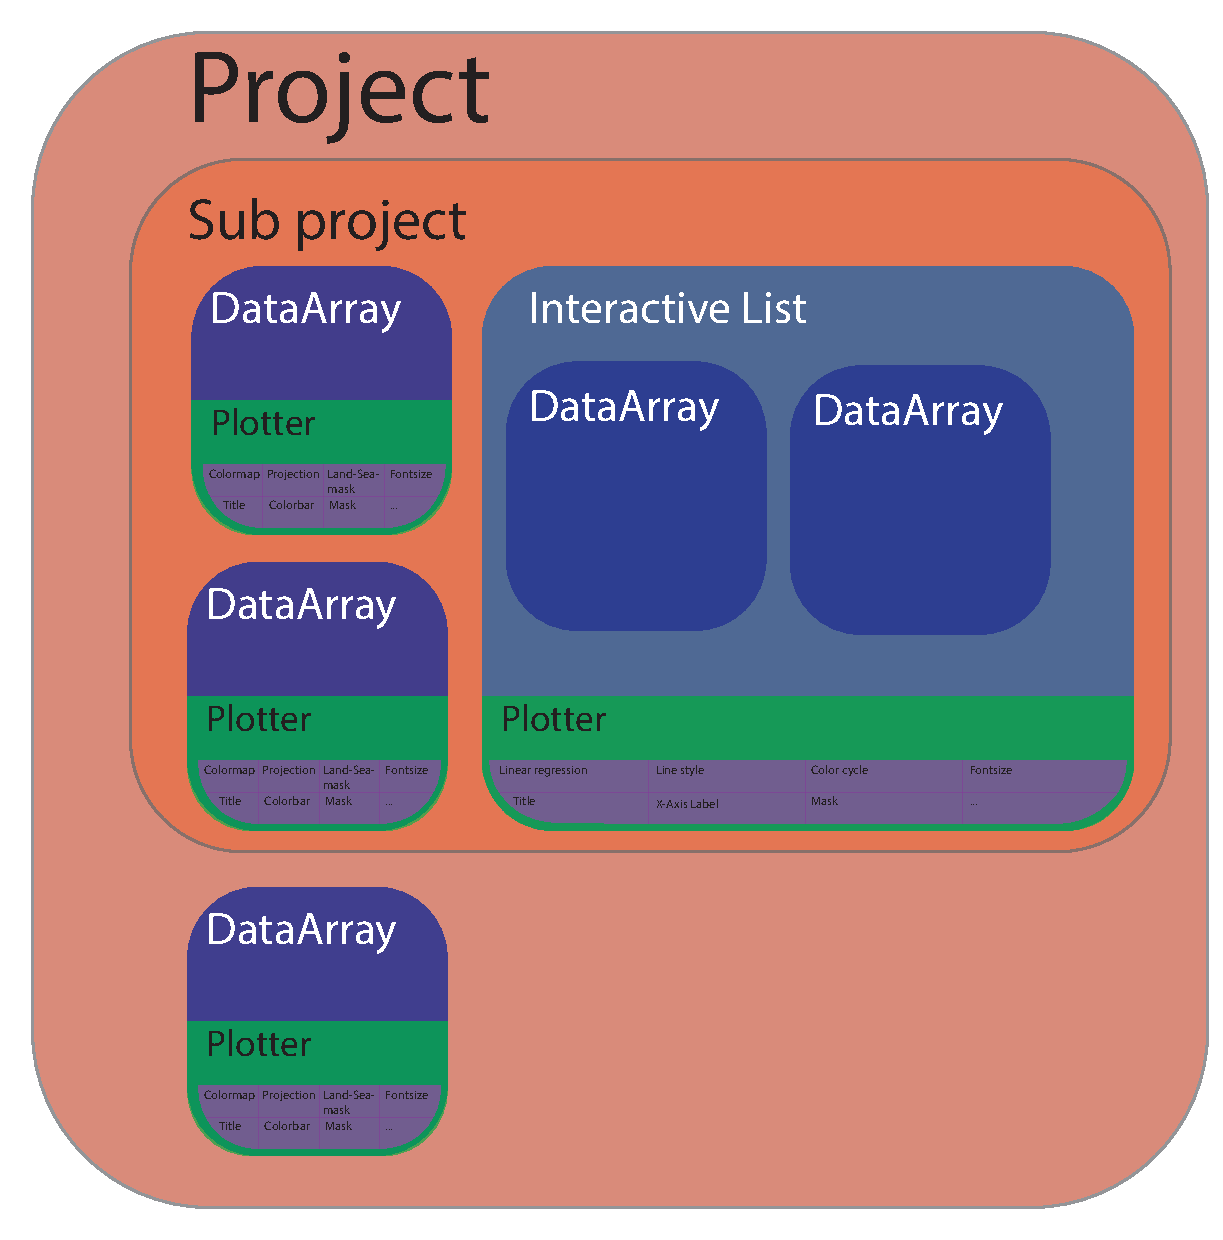
\includegraphics[width=\linewidth]{psyplot-figures/psyplot_framework.pdf}
	\caption[The psyplot core framework]{The psyplot core framework. A (sub) project consists of n-dimensional data arrays (in dark blue) or a list of these (in light blue) that are each visualized by a plotter (in green). Each plotter consists of a set of \textit{formatoptions} (in purple) that control the appearance of the plot or performs data manipulation or analysis.}
	\label{fig:psyplot-core}
\end{wrapfigure}

The next level is the \textit{DataArray} from the xarray package (or more explicitly, its accessor, the \textit{InteractiveArray}\footnote{\label{foot:xraccessors} several packages related to xarray are listed in the docs at \url{http://xarray.pydata.org/en/stable/related-projects.html} and psyplots integration (accessors) in particular is shown at \url{https://psyplot.github.io/psyplot/accessors.html}.}), that holds the data of one (or more) variables (e.g. temperature) and its corresponding coordinates (e.g. time, latitude, longitude, etc.). It may be one or multidimensional depending on the chosen visualization method. psyplot offers several methods to provide the coordinates for the plotting of different grids to make the visualization easier. The software can interpret CF Conventions\footnote{\url{http://cfconventions.org}} and UGRID conventions for unstructured grids \citep{JagersStuebeGrossEtAl2018}.

Multiple of these arrays can also be grouped together into an \textit{InteractiveList} that shall be visualized by the same plot method (e.g. multiple lines or a scalar field with overlying vector field).

The visualization part in the framework is managed by the \textit{Plotter} class, a collection of multiple \textit{Formatoptions}. Each plotter subclass is designed to visualize the data in a specific manner (e.g. via line plots, violin plots, or map plots) and is completely defined through it’s \textit{formatoptions}.

\textit{Formatoptions} are the core of the psyplot structure. The standard functionality of a formatoption is to control the visual appearance of one aspect of the plot (e.g. through the colormap, figure title, etc.). It is, however, completely unlimited and can also do data manipulations or calculations. The psy-reg plugin for example (see section \ref{sec:psyplot-plugins}) implements a formatoption that performs a regression through the data that is then visualized. As mentioned earlier, each plotter is set up through its \textit{formatoptions} where each formatoption has a unique formatoption key inside the plotter. This formatoption key (e.g. \textit{title} or \textit{cmap}) is what is used for updating the plot, manipulating the data, etc.. \textit{Formatoptions} might also interact with other \textit{formatoptions} inside the plotter or from other plotters. This concept of \textit{formatoptions} allows to use the same formatoption with all different kinds of plotters and the interaction of multiple plots with each other. Common plot features, such as the figure title, colormap, etc., therefore do not have to be implemented explicitly for every plotter but can be used from existing implementations. This framework also allows a very easy integration and development of own \textit{formatoptions} with a low or high level of complexity.

\subsection{Psyplot plugins}  \label{sec:psyplot-plugins}

The psyplot package provides the core of the data management described in the previous section \ref{sec:psyplot-core}. The real visualization is implemented in external plugins. The advantage of this approach is an increased flexibility of the entire framework (collaborations can evolve through dedicated plugins) and of managing the various dependencies of the packages. As such, the dependencies of psyplot are rather week (only xarray is needed), but the dependencies of the plugins can be more extensive (e.g. for geo-referencing or advanced statistics). 

Each plugin defines new \textit{Plotters} and \textit{Formatoptions} that are specific to the purpose of the visualization/analysis task. The plotters can also be implemented as a plot method and accessed through the psyplot core \gls{api} (see supplements \ref{sec:psyplot-example} for an example).

The current lists of plugins include \textit{psy-simple} for rather simple and standard visualization tasks, \textit{psy-maps} for geo-referenced plots, \textit{psy-reg} for statistical analysis visualization, and \textit{psy-strat} \citep{Sommer2019} for stratigraphic diagrams.

\subsubsection{psy-simple: The psyplot plugin for simple visualizations}

Much of the functionality that is used by other plugins is developed in the psy-simple plugin \citep{Sommer2017b}. This package targets simple visualizations and currently includes plot methods for one-dimensional data: line plots, bar plots and violin plots; for two-dimensional data: scalar plots, vector plots and combined scalar and vector plots; and plots that do not require complex data manipulation: a density plot and a plot of the weighted geographic mean.

This package also implements most of the functionality to handle unstructured grids in 2D visualizations and defines most of the commonly used \textit{formatoptions}. The latter include text manipulation (such as plot title, figure title, x- and y-axis labels, etc.), data masking, x- and y-axis tick labeling and positioning, as well as color coding for 2D plots (colormap, colormap sections, etc.).

\subsubsection{psy-maps: The psyplot plugin for visualizations on a map} \label{sec:psy-maps}

psy-maps \citep{Sommer2017c} builds on top of the psy-simple plugin and extends its functionality for visualizations on a map using the functionalities of the cartopy package \citep{Cartopy}. It simplifies as such the automated generation of maps for climate model data through the flexibility of the psyplot framework.

psy-maps currently implements additional \textit{formatoptions} for choosing the projection of the map, selecting the geographic region, drawing the contintens or shaded reliefs of land and ocean, and more. One feature that distinguishes psy-maps from other visualization software, even from pure cartopy, is the ability to visualize unstructured geo-referenced grids on the map such as in figure \ref{fig:unstructured-example}. The code to generate this left example\footnote{taken from \url{https://psyplot.github.io/examples/maps/example_ugrid.html}} shows the power of flexible \textit{formatoptions}:

\begin{Verbatim}[commandchars=\\\{\}]
\PY{n}{tsunami} \PY{o}{=} \PY{n}{psy}\PY{o}{.}\PY{n}{plot}\PY{o}{.}\PY{n}{mapplot}\PY{p}{(}
    \PY{l+s+s1}{\PYZsq{}}\PY{l+s+s1}{ugrid\PYZus{}demo.nc}\PY{l+s+s1}{\PYZsq{}}\PY{p}{,} \PY{n}{name}\PY{o}{=}\PY{l+s+s1}{\PYZsq{}}\PY{l+s+s1}{Mesh2\PYZus{}height}\PY{l+s+s1}{\PYZsq{}}\PY{p}{,} \PY{n}{load}\PY{o}{=}\PY{k+kc}{True}\PY{p}{,}
    \PY{c+c1}{\PYZsh{} formatoptions}
    \PY{n}{maskleq}\PY{o}{=}\PY{l+m+mi}{0}\PY{p}{,} \PY{n}{lonlatbox}\PY{o}{=}\PY{l+s+s1}{\PYZsq{}}\PY{l+s+s1}{Japan}\PY{l+s+s1}{\PYZsq{}}\PY{p}{,} \PY{n}{cmap}\PY{o}{=}\PY{l+s+s1}{\PYZsq{}}\PY{l+s+s1}{Blues}\PY{l+s+s1}{\PYZsq{}}\PY{p}{,} 
    \PY{n}{clabel}\PY{o}{=}\PY{l+s+s1}{\PYZsq{}}\PY{l+s+si}{\PYZob{}desc\PYZcb{}}\PY{l+s+s1}{\PYZsq{}}\PY{p}{,} \PY{n}{stock\PYZus{}img}\PY{o}{=}\PY{k+kc}{True}\PY{p}{,} \PY{n}{lsm}\PY{o}{=}\PY{l+s+s1}{\PYZsq{}}\PY{l+s+s1}{50m}\PY{l+s+s1}{\PYZsq{}}\PY{p}{,}
    \PY{n}{datagrid}\PY{o}{=}\PY{p}{\PYZob{}}\PY{l+s+s1}{\PYZsq{}}\PY{l+s+s1}{c}\PY{l+s+s1}{\PYZsq{}}\PY{p}{:} \PY{l+s+s1}{\PYZsq{}}\PY{l+s+s1}{k}\PY{l+s+s1}{\PYZsq{}}\PY{p}{,} \PY{l+s+s1}{\PYZsq{}}\PY{l+s+s1}{lw}\PY{l+s+s1}{\PYZsq{}}\PY{p}{:} \PY{l+m+mf}{0.1}\PY{p}{\PYZcb{}}
\PY{p}{)}
\end{Verbatim}


\begin{figure}
    \centering
    \includegraphics[width=0.45\linewidth]{campussource-figures/maps_example_ugrid_7_0.png}
    \includegraphics[width=0.45\linewidth]{campussource-figures/maps_example_ugrid_18_0.png}
    \caption{Example visualizations of a unstructured grids, taken from \href{https://psyplot.github.io/examples/maps/example_ugrid.html}{the example gallery}.}
    \label{fig:unstructured-example}
\end{figure}

\subsubsection{psy-reg: The psyplot plugin for visualizing and calculating regression plots}

psy-reg \citep{Sommer2017d} performs regression analysis on 1D variables using the methods of the stats-models \citep{SeaboldPerktold2010} and scipy \citep{JonesOliphantPetersonEtAl2001, Oliphant2007} packages, and visualizes the results with the functionalities of the psy-simple plugin. As such, it implements \textit{formatoptions} for univariate regressions, confidence intervals via bootstrapping, and combined plots of the data density and the fitted model. The necessity for this package arose from the need to visualize a regression model, compare it (visually) with the original data and to use it afterwards. Other python packages either focus only on the generation of the regressions (such as statsmodels or scipy), or on their visualization (such as seaborn \citep{WaskomBotvinnikOKaneEtAl2018}). The psyplot plugin makes it possible to generate the visualization and to access the underlying regression model parameters and uncertainties.

psy-reg has been heavily used for the parameterization of the which also gave the initial motivation for the package. 


\subsection{The psyplot Graphical User Interface}  \label{sec:psyplot-gui}

\begin{figure}
	\begin{tikzpicture}
		\node[anchor=south west,  inner sep=0] (image) at (0,0,0) {\includegraphics[width=\linewidth]{campussource-figures/psyplot-gui-screenshot.png}};
		\node[] (figures) [above=of image, xshift=-0.1\linewidth, yshift=-0.5cm, fill=red!50] {Figures};
		\node (project) [left=of figures, xshift=-0.1\linewidth, fill=red!50] {Project content};
		\node (help) [right=of figures, xshift=0.3\linewidth, fill=red!50] {Help explorer};
		\node (formatoptions) [below=of image, xshift=-0.1\linewidth, yshift=0.5cm, fill=red!50] {Formatoptions};
		\node (help) [right=of formatoptions, xshift=0.25\linewidth, fill=red!50] {psy-view interface};
		\node (console) [above=of formatoptions, yshift=1.5cm, fill=red!50] {Console};
	\end{tikzpicture}
%	\includegraphics[width=\linewidth]{psyplot-figures/psyplot-gui.png}
	\caption[Screenshot of the psyplot GUI]{Screenshot of the psyplot \gls{gui}. The left part shows the content of the psyplot project, the upper center the plots, and the right part contains the help explorer. Below the plots, there is also the IPython console for the usage from the command line and a widget to update the \textit{formatoptions} of the current project.}
	\label{fig:psyplot-gui}
\end{figure}

\begin{figure}
	\centering
	\includegraphics[width=0.7\linewidth]{psyplot-figures/plot-creator.png}
	\caption[psyplot Gui plot creation dialog]{Plot creation dialog to generate new figures from an xarray dataset.}
	\label{fig:psyplot-gui-plot-creator}
\end{figure}

Psyplots objective of providing a platform for flexible and convenient data analysis is further approached with the \textit{psyplot-gui} package. This extension to the framework provides a \gls{gui} for simplified access to the plotting features in psyplot.

A strong focus of this interface is, again, the flexibility. psyplot-gui is based on the cross-platform PyQt5 library\footnote{PyQt5 can be accessed via \url{https://riverbankcomputing.com/software/pyqt/intro}.}, a very flexible and frequently used package for \acrlongpl{gui}. This enables other software to develop additional features for the package (see psy-strat in the previous section \ref{sec:psyplot-plugins}, for instance, or straditize \citep{SommerRechChevalierEtAl2019}) and to flexibly change the layout of the application. The \gls{gui} is complemented with an interactive console to provide a fully integrated python environment for data analysis.

The next paragraphs provide an overview on the various widgets, that are also displayed in figure \ref{fig:psyplot-gui} and \ref{fig:psyplot-gui-plot-creator}. 

\subsubsection{Console}
The central aspects to guarantee flexibility of the application is an in-process IPython console, based on the qtconsole package\footnote{\url{https://github.com/jupyter/qtconsole}} that provides the possibility to communicate with the psyplot package via the command line and to load any other module or to run any other script or notebook, or even to run commands in different programming languages, such as R \citep{RCT2019} or Julia \citep{BezansonEdelmanKarpinskiEtAl2017}. The console is fully integrated both ways into the \gls{gui}. The documentation of every python object in the terminal, for instance, can be viewed in the help explorer of the GUI. And vice versa: a change of the current project through the project content widgets, also changes the corresponding python variable in the shell. 

\subsubsection{psy-view}
psy-view \citep{Sommer2021} is a relatively new interface build upon the psyplot framework for a quick visualization of netCDF files. It runs as a stand-alone software, but additionally as a plugin for the general psyplot \gls{gui}. psy-view provides quick functionalities to open datasets, select and visualize four-dimensional variables, change the dimensions such as time or vertical level, and update the appearance of the plot, e.g. the projection, title or color coding. 

psy-view has been inspired by ncview\footnote{\url{http://meteora.ucsd.edu/~pierce/ncview_home_page.html}}, that provides an equally simple design. The major difference between the two software packages is that psy-view also supports the visualization of unstructured grids as it's using the visualizations of the psy-maps package (\ref{sec:psy-maps})\footnote{A more detailed comparison between psy-view and ncview can be found at \url{https://psyplot.github.io/psy-view/ncview.html}.}.

\subsubsection{Help explorer}
As a complement to the console, the \gls{gui} contains a help explorer to provide immediate and dynamic access to the documentation of python objects in the console, rendered as an HTML webpage\footnote{The help explorer widget has been originally motivated by the \textit{Help} widget of the Scientific PYthon Development EnviRonment, Spyder (\url{https://www.spyder-ide.org/}) and uses the sphinx package \citep{Hasecke2019} to convert restructured Text into HTML.}. Furthermore, the help explorer is connected to multiple other widgets of the \gls{gui} in order to provide a dynamically generated documentation. The documentation of available \textit{formatoptions} in the psyplot project, for instance, are rendered as HTML upon request, in order to make the various plot methods more accessible. The same principle works for the plot methods that are accessible in the plot creator.

\subsubsection{Plot creator}
The plot creator (figure \ref{fig:psyplot-gui-plot-creator}) is the starting point of the \gls{gui} into the psyplot framework (at least, if one does not use the console or a script to generate the plots). It loads data from the disk or the in-process console, and essentially provides a wrapper around the psyplot plotting call (see suppl. section \ref{sec:psyplot-example}). It additionally displays the documentation of the method and its associated \textit{formatoptions}. This widget creates new plots, that are appended to the psyplot project and are accessible through the console and the project content widgets.

\subsubsection{Project content}
The psyplot project is the most high-level \gls{api} element in the psyplot framework (see section \ref{sec:psyplot-core}) and is displayed in the project content widgets of the \gls{gui}. All other elements, such as the \textit{formatoptions} widget or the plot creator, are interfering with the project, and it is accessible as a variable in the console. The project content widget can be used to see the various items in the project, but it is also used to select the specific items for the so-called \textit{current} sub-project. The latter is dynamically set in the console through the \texttt{sp} variable and it is used by the \textit{formatoptions} widget to update the plotting parameters of the selected items.

\subsubsection{Formatoptions}
As mentioned in section \ref{sec:psyplot-core}, \textit{formatoptions} are the core elements in psyplot that control the figure aesthetics of the plots and/or perform data manipulations. The generic \textit{formatoptions} widget provides access to these parameters, in order to update them for the selected items in the current project. The formatoption itself (i.e. the python object) can in turn generate a widget that is implemented in the \textit{formatoptions} widget, to make the available options more accessible. The \textit{title} formatoption, for instance, generates a drop-down menu to select variable attributes (e.g. variable name, variable units, etc.) which is then embedded in the \textit{formatoptions} widget. The modifications of the \textit{formatoptions} via this widgets, updates the figures of the selected items.

\subsubsection{Figures and plots}
The plots generated by the plotting methods are displayed in dedicated widgets inside the \gls{gui} and can be dynamically adjusted using the \textit{formatoptions} widget or the console. The underlying library of the current implemented psyplot plugins, matplotlib, implements multiple backends to display the data interactively, or to export them as PDF, PNG, etc. The psyplot \gls{gui} has implemented a backend on top of the PyQt5 backend of matplotlib, which embeds the figures in the \gls{gui}. psyplot can, however, work with any backend of matplotlib and does not depend on the specific implementation.

\section{Conclusions}  \label{sec:psyplot-conclusions}
psyplot \citep{Sommer2017} is a flexible framework that integrates rich computational and mathematical software into a flexible framework for data analysis and visualization. The design of the high-level API of the framework enables a simple and standardized usage from the command-line, python scripts or jupyter notebooks. A modular plugin framework enables a flexible development of the framework that can potentially go into many different directions. The additional enhancement with a flexible \gls{gui} makes it the only visualization framework that can be handled conveniently from the command-line, and via point-click handling. It also allows to build further desktop applications on top of the existing framework. The recently developed psy-view package further extends these functionalities with an easy-to-use \gls{gui} for data visualization.

psyplot provides a framework that can be adapted by scientists. This improves reproducibility and maintainability of research software, and encourages scientists to split their analysis into modular pieces that can be better tested and reused.

Scientists can further build upon a variety of existing visualization options provided by different plugins. They currently provide visualization methods that range from simple line plots, to density plots, regression analysis and geo-referenced visualization in two dimensions. The software is currently entirely based on the visualization methods of matplotlib \citep{Hunter2007}, the most established visualization package in the scientific python community. However, the framework itself is agnostic to the underlying visualization method and can, as such, leverage a variety of existing analytical software.


\clearpage

\begin{subappendices}
	\section*{Supplementary material}
	\section{Example call of a plot method}  \label{sec:psyplot-example}
	
	\begin{Verbatim}[commandchars=\\\{\}]
\PY{c+c1}{\PYZsh{} example call for generating a map}
\PY{k+kn}{import} \PY{n+nn}{psyplot.project} \PY{k+kn}{as} \PY{n+nn}{psy}

\PY{n}{maps} \PY{o}{=} \PY{n}{psy}\PY{o}{.}\PY{n}{plot}\PY{o}{.}\PY{n}{mapplot}\PY{p}{(}
    \PY{l+s+s1}{\PYZsq{}}\PY{l+s+s1}{psy\PYZhy{}maps\PYZhy{}demo.nc}\PY{l+s+s1}{\PYZsq{}}\PY{p}{,}  \PY{c+c1}{\PYZsh{} input file name, can also be data in memory}
    \PY{n}{name}\PY{o}{=}\PY{l+s+s1}{\PYZsq{}}\PY{l+s+s1}{t2m}\PY{l+s+s1}{\PYZsq{}}\PY{p}{,}          \PY{c+c1}{\PYZsh{} variable to plot (can also be multiples}
    \PY{c+c1}{\PYZsh{}\PYZsh{}\PYZsh{} formatoptions}
    \PY{c+c1}{\PYZsh{} colorbar label uses meta attributes of netCDF variable}
    \PY{n}{clabel}\PY{o}{=}\PY{l+s+s1}{\PYZsq{}}\PY{l+s+si}{\PYZpc{}(long\PYZus{}name)s}\PY{l+s+s1}{ [}\PY{l+s+si}{\PYZpc{}(units)s}\PY{l+s+s1}{]}\PY{l+s+s1}{\PYZsq{}}\PY{p}{,}
    \PY{c+c1}{\PYZsh{} select colormap}
    \PY{n}{cmap}\PY{o}{=}\PY{l+s+s1}{\PYZsq{}}\PY{l+s+s1}{RdBu\PYZus{}r}\PY{l+s+s1}{\PYZsq{}}\PY{p}{,}
    \PY{c+c1}{\PYZsh{} focus on a specific lonlatbox given by [lonmin, lonmax, latmin, latmax]}
    \PY{n}{lonlatbox}\PY{o}{=}\PY{p}{[}\PY{l+s+s1}{\PYZsq{}}\PY{l+s+s1}{Europe}\PY{l+s+s1}{\PYZsq{}}\PY{p}{,} \PY{l+s+s1}{\PYZsq{}}\PY{l+s+s1}{Europe}\PY{l+s+s1}{\PYZsq{}}\PY{p}{,} \PY{l+m+mi}{0}\PY{p}{,} \PY{l+s+s1}{\PYZsq{}}\PY{l+s+s1}{Europe}\PY{l+s+s1}{\PYZsq{}}\PY{p}{]}\PY{p}{)}

\PY{n}{maps}\PY{o}{.}\PY{n}{show}\PY{p}{(}\PY{p}{)}
\end{Verbatim}
  % generated with pygmentize -o example_call.text example_call.py
	\includegraphics[width=0.45\linewidth]{psyplot-figures/example-call.pdf}
	
	\begin{Verbatim}[commandchars=\\\{\}]
\PY{c+c1}{\PYZsh{} Update the plot, e.g. change projection, plot global}

\PY{n}{maps}\PY{o}{.}\PY{n}{update}\PY{p}{(}\PY{n}{projection}\PY{o}{=}\PY{l+s+s1}{\PYZsq{}}\PY{l+s+s1}{robin}\PY{l+s+s1}{\PYZsq{}}\PY{p}{,} \PY{n}{lonlatbox}\PY{o}{=}\PY{n+nb+bp}{None}\PY{p}{)}
\end{Verbatim}

	\includegraphics[width=0.6\linewidth]{psyplot-figures/example-update.pdf}

\end{subappendices}\

\clearpage

\printnoidxglossary[type=acronym, title={List of Abbreviations}]

\printbibliography

\end{refsection}

%----------------------------------------------------------------------------------------
%	SYMBOLS
%----------------------------------------------------------------------------------------

%\begin{symbols}{lll} % Include a list of Symbols (a three column table)
%
%	$a$ & distance & \si{\meter} \\
%	$P$ & power & \si{\watt} (\si{\joule\per\second}) \\
%	%Symbol & Name & Unit \\
%
%	\addlinespace % Gap to separate the Roman symbols from the Greek
%
%	$\omega$ & angular frequency & \si{\radian} \\
%
%\end{symbols}

% Include the appendices of the thesis as separate files from the Appendices folder
% Uncomment the lines as you write the Appendices

%% List of publications

\chapter{Publications and Conference contributions} % Main appendix title

\label{chp:pub}
\subsection{Peer-reviewed}

\begin{refsection}[papers.bib]
	\begin{refcontext}[sorting=ydnt]
		\nocite{*}
		\printbibliography[heading=none]
	\end{refcontext}
\end{refsection}


\subsection{Conference contributions}

\begin{refsection}[conferences.bib]
	\begin{refcontext}[sorting=ydnt]
		\nocite{*}
		\printbibliography[heading=none]
	\end{refcontext}
\end{refsection}
%% An overview on software packages developed during the PhD

\chapter{New Software Tools - An Overview}

\label{chp:software}

This section mainly contains the latest version of the package, a short
summary and an information table about where to find everything
(Documentation, source code, etc.)

\todo[inline]{Need to write chapter \ref{chp:software}}


\section{Main packages} \label{sec:software-main}

\begin{itemize}
	\item psyplot
	\begin{itemize}
		\item psy-simple
		\item psy-maps
		\item psy-reg
		\item psyplot-gui
		\item psy-strat
	\end{itemize}
	\item straditize
	\item gwgen
	\item iucm
	\item EMPD
	\begin{itemize}
		\item EMPD-admin
		\item EMPD-viewer
		\item EMPD-data
	\end{itemize}
	\item POLNET
	\begin{itemize}
		\item POLNET-viewer
		\item POLNET-data
	\end{itemize}	
\end{itemize}


\section{Other packages} \label{sec:software-others}

\begin{itemize}
	\item docrep
	\item sphinx-nbexamples
	\item model-organization
	\item funcargparse
	\item autodocsumm
\end{itemize}

%----------------------------------------------------------------------------------------

\end{document}
